\section{Hình ảnh và biểu đồ, công cụ để biểu diễn khoa học}

\ 

Như đã viết, con người tiếp nhận hình ảnh nhanh hơn nhiều so với câu chữ. Khẳng định này có khi không cần phải chứng minh, những chúng ta vẫn hãy lấy một ví dụ, như ở hình \ref{fig:khoa_hoc:gioi_thieu_ngan:hinh_cong_cu:dong_ho_trong_tuyet}.

\begin{figure}[H]
   \centering
   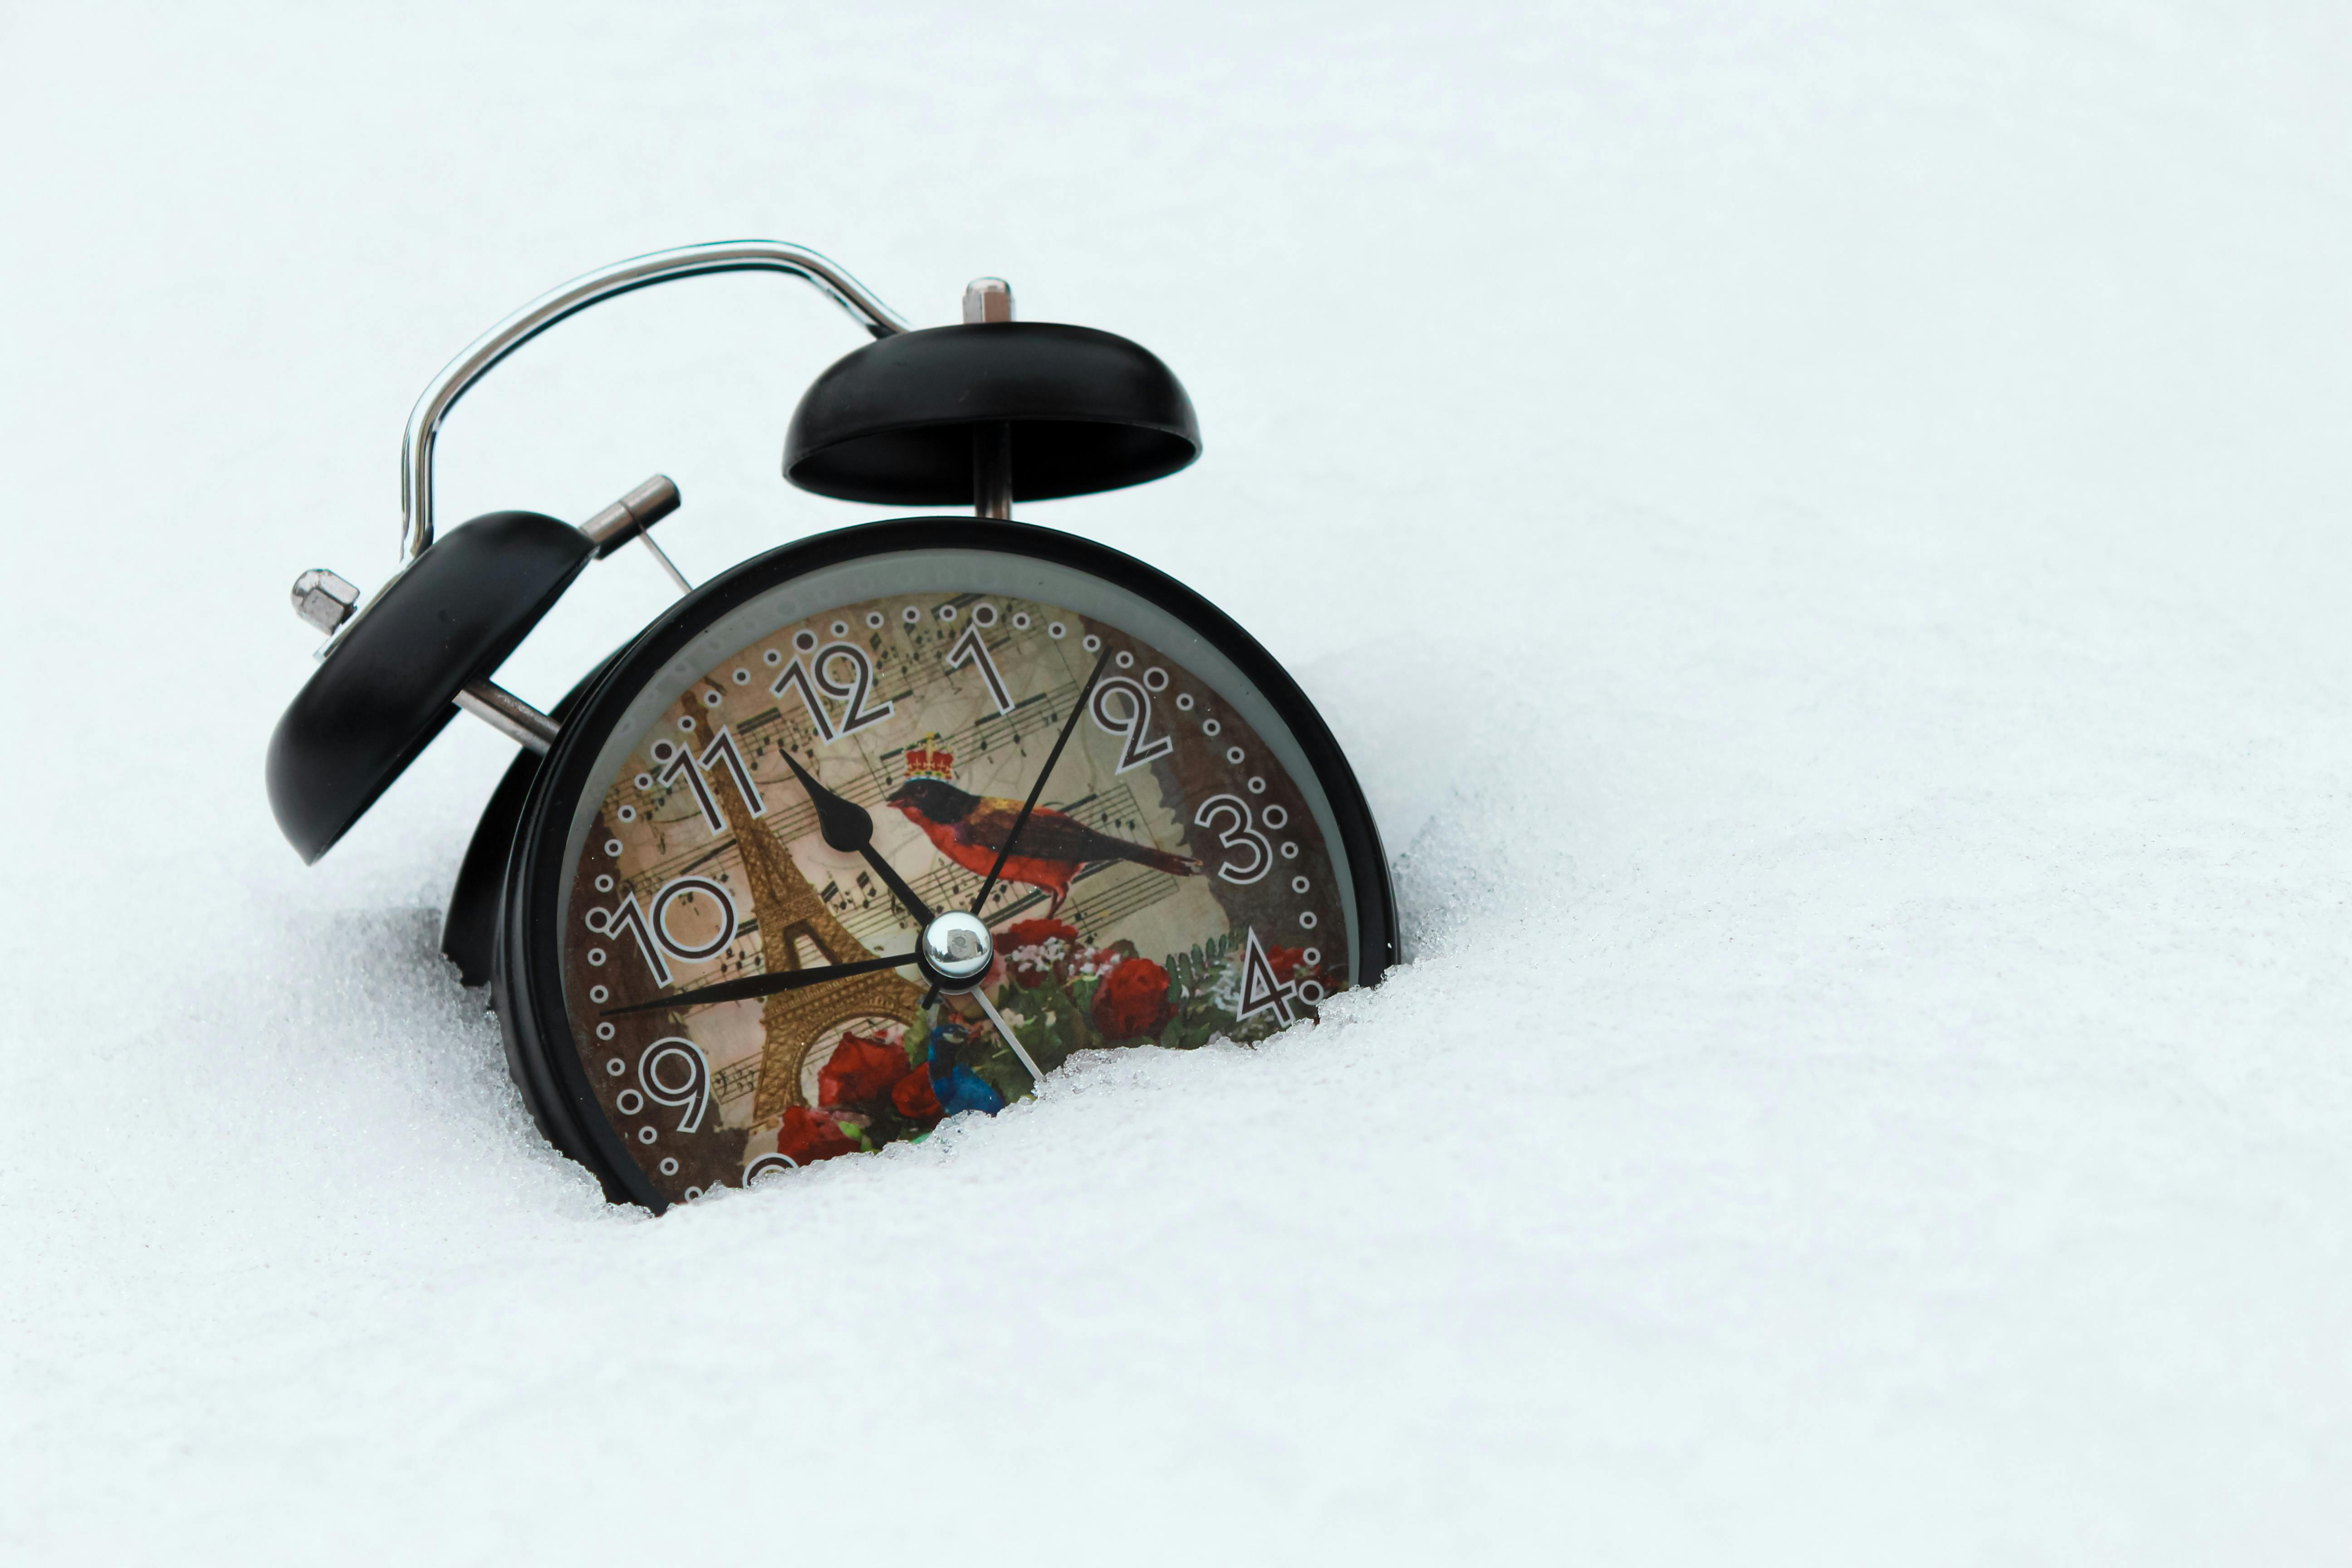
\includegraphics[width=0.8\textwidth]{images/dong_ho_trong_tuyet.jpg}
   \caption{Một chiếc đồng hồ báo thức bị vùi trong tuyết mùa đông.\\Nguồn: https://www.pexels.com/photo/black-alarm-clock-on-snow-covered-ground-10976666/}
   \label{fig:khoa_hoc:gioi_thieu_ngan:hinh_cong_cu:dong_ho_trong_tuyet}
\end{figure}

Thấy được ngay chú thích một dòng ``Một chiếc đồng hồ báo thức bị vùi trong tuyết mùa đông.'' mới chỉ tóm tắt sơ bộ những sự vật xuất hiện trong ảnh. Với một số quan sát, chúng ta có thể mô tả cụ thể đồng hồ hơn như:
\begin{itemize}
   \item Đồng hồ có thiết kế cơ khí cổ điển với hai chuông, vỏ ngoài màu đen, chuông đen và tay cầm bằng kim loại cong màu crôm hoặc bạc nối hai chuông ở phía trên.
   \item Đồng hồ hơi nghiêng sang trái, tựa lưng vào đống tuyết. Nửa dưới thân đồng hồ chìm trong tuyết.
   \item Mặt đồng hồ có thiết kế nghệ thuật. Nó có kết cấu giấy trông như giấy cũ, được phủ các nốt nhạc. Trên đó là những hình minh họa đầy màu sắc: tháp Ép-phen (Eiffel) ở bên trái, một con chim màu đỏ và đen rực rỡ (giống chim sẻ hoặc chim hồng tước) đậu gần giữa bên phải, và một cụm hoa hồng đỏ ở phía dưới.
   \item Các con số được đánh dấu bằng các chữ số Ả Rập màu đen viền trắng theo phông không chân. Các nốt tròn cũng nền đen viền trắng chấm chạy dọc theo mép ngoài cùng để biểu thị vị trí cho kim phút và giây. Chiếc đồng hồ có ba kim màu đen gặp nhau ở một chốt bạc trung tâm.
\end{itemize}

Bạn đọc có thể miêu tả chiếc đồng hồ hay hơn tác giả, nhưng để làm được điều đó mà không hi sinh các chi tiết, ít nhiều cũng phải dùng một lượng từ vựng tương đường hoặc gấp nhiều lần con số khoảng 150 từ trong ví dụ tác giả đưa ra. Và dù chúng ta cố gắng viết một bài văn thuyết minh chiếc đồng hồ này cụ thể, tỉ mỉ, và chính xác đến thế nào đi chăng nữa, khi chúng ta đưa bài văn đó cho \num{9} người họa sĩ và bảo họ vẽ một bức tranh, chúng ta sẽ nhận lại được \num{10} bức tranh khác nhau, và chắc chắn sẽ khác bức hình \ref{fig:khoa_hoc:gioi_thieu_ngan:hinh_cong_cu:dong_ho_trong_tuyet} mà chúng ta đã có ở ban đầu.

Vậy, tại sao một hình ảnh lại có thể truyền đạt nhiều thông tin đến như vậy? Câu trả lời nằm ở việc chúng ta hiểu rõ các sự vật xuất hiện và hiện tượng xảy ra trong bức hình. Với con người ở thế kỉ \Rmnum{21}, có lẽ người ta không xa lạ gì với chiếc đồng hồ báo thức, tháp bằng thép nổi tiếng nhất của Pháp, hay tiếng hót của những chú chim. Dù chúng ta có thể chưa bao giờ cầm nắm chiếc đồng hồ ở hình \ref{fig:khoa_hoc:gioi_thieu_ngan:hinh_cong_cu:dong_ho_trong_tuyet}, với sự tiếp xúc vốn có với thế giới, chúng ta có thể tự tưởng tượng ra hình ảnh chiếc đồng hồ và cảm nhận của chúng ta về nó.

Tuy nhiên, đây cũng có thể là một hạn chế của tranh ảnh, khi phụ thuộc vào khả năng nhận thức của con người. Bạn đọc có thể thấy giới hạn của trí tưởng tượng khi đọc đến hai ví dụ sau (nếu như bạn đọc chưa biết về chủ nghĩa duy vật lịch sử):
\begin{itemize}
   \item ``Cơ sở hạ tầng là toàn bộ những quan hệ sản xuất của một xã hội trong sự vận động hiện thực của chúng hợp thành cơ cấu kinh tế của xã hội đó.'';
   \item ``Kiến trúc thượng tầng là toàn bộ những quan điểm, tư tưởng xã hội với những thiết chế xã hội tương ứng cùng những quan hệ nội tại của thượng tầng hình thành trên một cơ sở hạ tầng nhất định.''.
\end{itemize}
Đây là định nghĩa tác giả trích từ \cite{djc2024giao}. Kể cả khi bạn đọc chưa hiểu rõ về hai khái niệm này, tác giả đoán rằng bạn đọc đã có một chút định hướng, và nếu tìm hiểu sâu thêm, có thể bạn đọc sẽ có sự thông hiểu cần thiết và góc nhìn sâu sắc để phát hiện tính biện chứng giữa chúng. Liệu bạn đọc có được sự định hướng ban đầu đó nếu tác giả đưa hai hình ảnh minh họa cho hai khái niệm này? Hoặc, câu hỏi quan trọng hơn, cần phải ``vẽ'' ra sao để không làm mất nghĩa? 